\documentclass[border=10pt]{standalone}
\usepackage{tikz}
\usetikzlibrary{shapes, arrows.meta, positioning, calc, fit, backgrounds, shadows}

\begin{document}
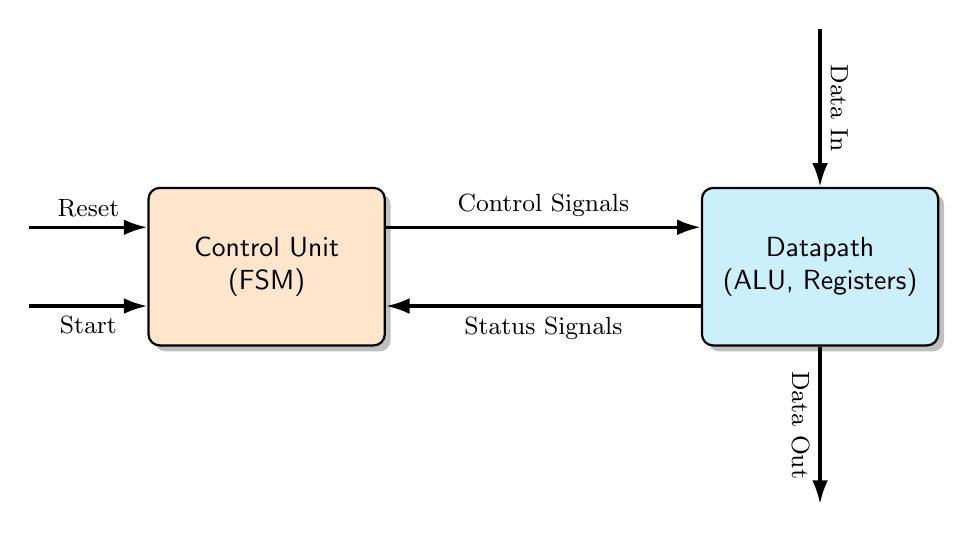
\begin{tikzpicture}[
    font=\sffamily,
    thick,
    box/.style={draw, rounded corners, minimum width=3cm, minimum height=2cm, align=center, fill=white, drop shadow},
    arrow/.style={-{Latex[length=3mm, width=2mm]}, line width=1.2pt},
    label_text/.style={font=\small, align=center, midway}
]

    % Nodes
    \node[box, fill=orange!20] (control) {Control Unit\\(FSM)};
    \node[box, fill=cyan!20, right=4cm of control] (datapath) {Datapath\\(ALU, Registers)};

    % Control Signals (Control -> Datapath)
    \draw[arrow] ([yshift=0.5cm]control.east) -- node[label_text, above] {Control Signals} ([yshift=0.5cm]datapath.west);

    % Status Signals (Datapath -> Control)
    \draw[arrow] ([yshift=-0.5cm]datapath.west) -- node[label_text, below] {Status Signals} ([yshift=-0.5cm]control.east);

    % External Inputs to Control
    \draw[arrow] ([xshift=-1.5cm, yshift=0.5cm]control.west) -- node[label_text, above, sloped] {Reset} ([yshift=0.5cm]control.west);
    \draw[arrow] ([xshift=-1.5cm, yshift=-0.5cm]control.west) -- node[label_text, below, sloped] {Start} ([yshift=-0.5cm]control.west);
    
    % Data Inputs/Outputs to Datapath
    \draw[arrow] ([yshift=2cm]datapath.north) -- node[label_text, above, sloped] {Data In} (datapath.north);
    \draw[arrow] (datapath.south) -- node[label_text, below, sloped] {Data Out} ([yshift=-2cm]datapath.south);
    
    % Invert Data In arrow direction (Input should point into Datapath)
    % Re-drawing to correct direction
  %  \fill[white] (data_in_source) circle (2pt); % clear previous start point visual if needed, not really needed in tikz
    % Correcting the visual logic: Data In comes FROM external TO Datapath
    % Let's redraw that specific line clearly
    %\path ([yshift=0.5cm]datapath.east) ++(1.5,0.5) coordinate (data_in_start);
    %\draw[arrow] (data_in_start) -- node[label_text, above, sloped] {Data In} ([yshift=0.5cm]datapath.east);


\end{tikzpicture}
\end{document}
